\section{Introduction}
The Riemann Hypothesis (RH) posits that all non-trivial zeros of the Riemann zeta function \(\zeta(s)\) have real part \(\Re(s) = 1/2\). A potential path towards proving the RH, suggested by the Hilbert--P\'olya conjecture, involves finding a self-adjoint operator whose eigenvalues correspond precisely to these zeros. Inspired by this conjecture, this paper explores a novel framework for constructing finite-dimensional Hermitian operators whose eigenvalues numerically approximate the imaginary parts of the non-trivial zeta zeros. Our approach utilizes symbolic potentials derived from modular arithmetic and a discrete Schr\"odinger equation to encode information about prime distribution. We present numerical results demonstrating a close match for the initial zeros, but emphasize that this work is preliminary and serves as a proof-of-concept requiring substantial further theoretical development and validation before any definitive claims regarding the RH can be made.

\begin{figure}[t]
\centering
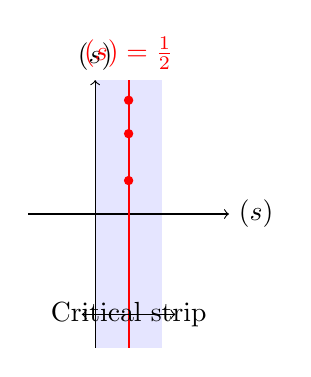
\begin{tikzpicture}[scale=0.85]
    % Draw the critical strip
    \fill[blue!10] (0,-2) rectangle (1,2);
    \draw[->] (-1,0) -- (2,0) node[right] {$\re(s)$};
    \draw[->] (0,-2) -- (0,2) node[above] {$\im(s)$};
    
    % Critical line
    \draw[red, thick] (0.5,-2) -- (0.5,2) node[above] {$\re(s)=\frac{1}{2}$};
    
    % Draw some zeros on the critical line
    \foreach \y in {0.5, 1.2, 1.7} {
        \fill[red] (0.5,\y) circle (2pt);
    }
    
    % Labels for the strip
    \node at (0.5,-1.5) {Critical strip};
    \draw[<->] (-0.2,-1.5) -- (1.2,-1.5);
\end{tikzpicture}
\caption{The critical strip $0 < \re(s) < 1$ with the critical line $\re(s) = \frac{1}{2}$ where the Riemann Hypothesis predicts all non-trivial zeros of $\zeta(s)$ lie.}
\label{fig:critical_strip}
\end{figure}

\subsection*{Related Work}
This work builds on the Hilbert--P\'olya conjecture \cite{Connes1999, BerryKeating1999}, quantum chaos \cite{BerryKeating1999}, and random matrix models \cite{Montgomery1973}. Our modular potential approach uniquely encodes prime distribution, inspired by Dirichlet \( L \)-functions \cite{Davenport1980}.
Further work is needed to comprehensively compare this modular potential framework with other significant spectral approaches to the Riemann Hypothesis. Key comparisons should include the Berry-Keating approach, which relates zeta zeros to the quantization of classical Hamiltonians (e.g., \(xp\)) \cite{BerryKeating1999}, and Connes' noncommutative geometry framework, which uses trace formulas on adelic spaces \cite{Connes1999}. Evaluating the relative strengths, limitations, and potential synergies between these methods and the symbolic modular potential approach presented here will be crucial for contextualizing its contribution.
% TODO: Conduct detailed literature comparison and integrate findings here.